\label{sez:interfaccia}

\begin{figure}[]
	\centering
	%\def\svgwidth{0.7\linewidth}
	%\input{schema_2.pdf_tex}
	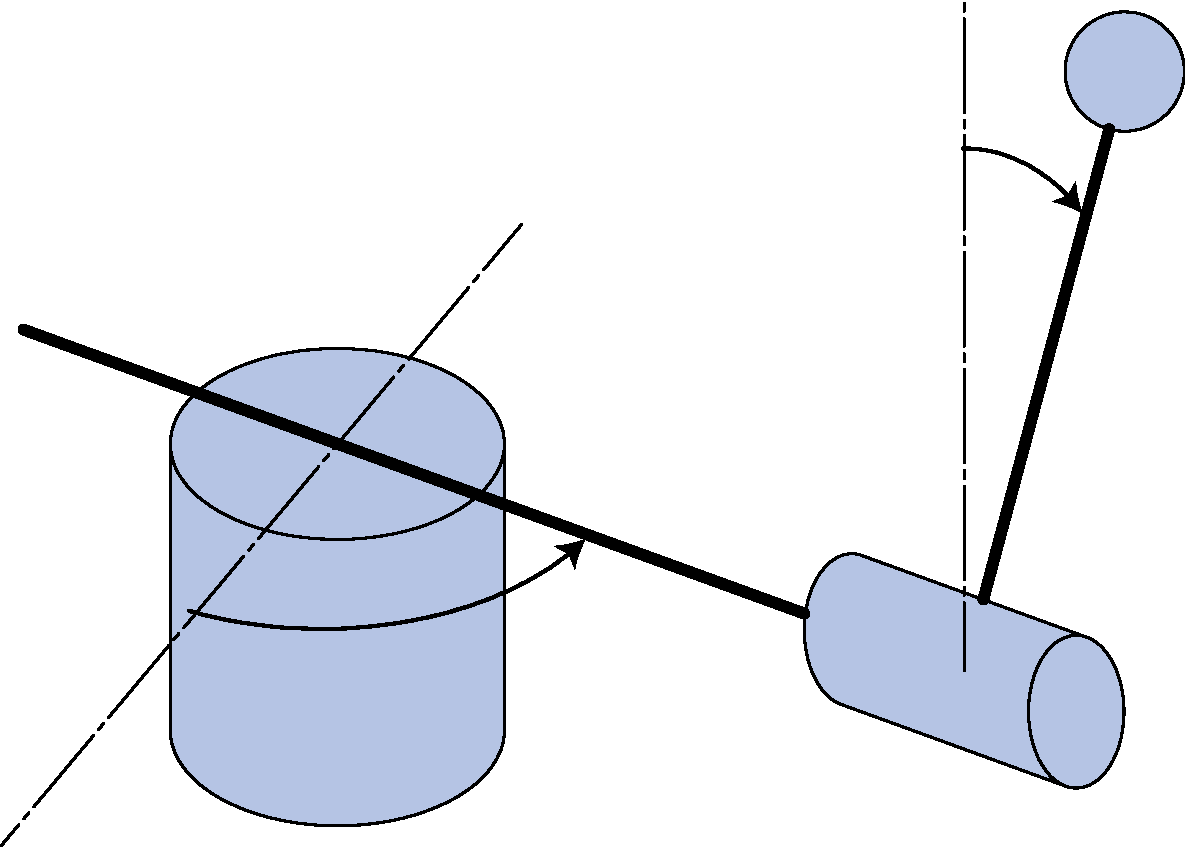
\includegraphics[width=.7\linewidth]{schema_2.pdf}
	\caption{Schema del Pendolo \textbf{DA SISTEMAREE}}
	\label{fig:pendolo_schema}
\end{figure}

\begin{figure}[]
	\centering
	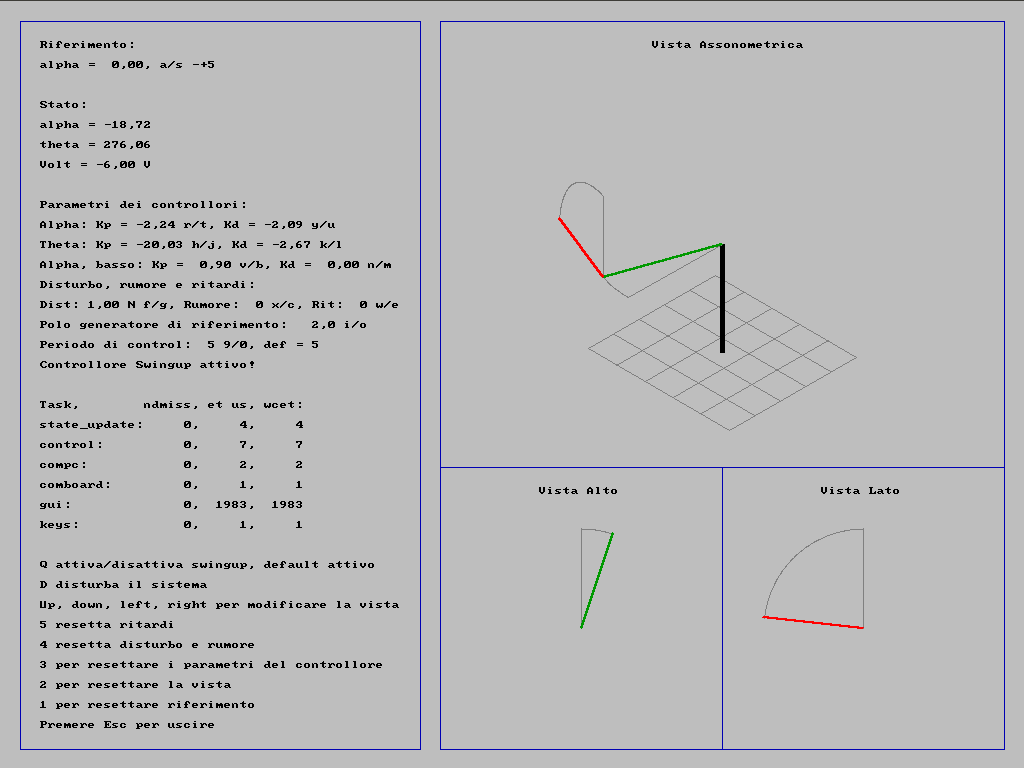
\includegraphics[height=.4\textheight]{interfaccia_in_esecuzione.png}
	\caption{Interfaccia durante l'esecuzione}
	\label{fig:interfaccia_in_esecuzione}
\end{figure}
L'interfaccia \`e divisa in due zone principali: quella di comunicazione con l'utente e le tre viste del pendolo.
Per quanto riguarda la zona di comunicazione questa \`e popolata dalle variabili di interesse e di come modificarle. Si \`e quindi riportato a schermo:
\begin{itemize}
	\item il riferimento su $\alpha$
	
	\item  il vettore di stato $\left[ \alpha \ \theta \ volt\right]^T$
	
	\item i parametri di controllo
	
	\item disturbo, rumore e ritardi
	
	\item polo della funzione di trasferimento che genera il riferimento su $\alpha$
	
	\item periodo del task di controllo
	
	\item per ciascun task il numero di deadline miss, il tempo di esecuzione in $\si{\micro \second}$ e il worst-case execution time in $\si{\micro \second}$
	
	\item varie istruzioni su come resettare e come uscire dal programma
	
\end{itemize}
Per quanto riguarda le viste, queste sono tre. La vista dall'alto evidenzia il primo link e quindi \`e possibile vedere $\alpha$ mentre in quella da lato $\theta$.

Per costruire la vista assonometrica \`e stato utile strutturare il problema in coordinate omogenee e introdurre dei sistemi di riferimento ausiliari. Tenendo d'occhio la figura~\ref{fig:pendolo_schema} e intendendo con $R_i(\varphi)$ la generica rotazione intorno all'asse $i$ di un angolo $\varphi$ e con $T_{ij}$ la trasformazione in coordinate omogenee dal sistema di riferimento $i$ a quello $j$ tale che per un generico vettore $p$ valga: $^ip = T_{ij}\ ^j p$; si pu\`o elaborare i cambi di coordinate necessari. 
\begin{equation}
	^0\! T_{01}(\alpha) = \left[ \begin{array}{ccc|c}
	& & & l_1 \\
	& R_z(\alpha) & & 0 \\
	& & & 0 \\
	\hline
	0 & 0 & 0 & 1
	\end{array} \right]
	\quad 
	^1 T_{12}(\vartheta) =
	\left[  \begin{array}{ccc|c}
	& & & 0 \\
	& R_x(\theta) & & 0 \\
	& & & 0 \\
	\hline
	0 & 0 & 0 & 1
	\end{array}
	\right]
\label{eq:cambio_coordinate}
\end{equation}
Quindi si possono ricavare le coordinate in sistema di riferimento $0$ dei punti di interesse:
\begin{equation}
	\begin{aligned}
		^0\! \mathrm{OA}& =\ ^0\!T_{01}(\alpha) \begin{bmatrix} 0& 0 & 0& 1 \end{bmatrix}^t\label{eq:from_punti_in_coord_0} \\
		^0\! \mathrm{AP}& = \ ^0\! T_{12}(\vartheta)
		\left[  \begin{array}{ccc|c}
		& & & 0 \\
		& Id & & 0 \\
		& & & l_2 \\
		\hline
		0 & 0 & 0 & 1
		\end{array}
		\right] \\
		^0\! \mathrm{OP}& = \ ^0\! \mathrm{OA}+\ ^0\! \mathrm{AP}
	\end{aligned}
\end{equation}
e in forma estesa:
\begin{equation}
	\begin{aligned}
	^0\!\mathrm{OA} = &\left[ \begin{array}{c} l_1 \cos\alpha \\ l_1 \sin \alpha \\ 0 \end{array}\right] \\
	^0\!\mathrm{OP} = &\left[ \begin{array}{c} l_1 \cos \alpha - l_2 \sin \alpha \sin \vartheta\\ l_1 \sin \alpha + l_2 \cos \alpha \sin \vartheta\\ l_2 \cos \vartheta \end{array}\right]
	\end{aligned}
\end{equation}
Per poi ottenere le coordinate di un punto qualsiasi  nell'interfaccia \`e sufficiente proiettare nel piano usando la seguente relazione, indicando con $s$ gli assi assonometrici, con $\rho$ l'angolo di longitudine e con $\lambda$ quello di latitudine:
\begin{equation}
	R_{s0} = R_z (\rho)  R_y (-\lambda)  \begin{bmatrix}
	0 & 0 & -1\\
	1 & 0 & 0\\
	0 & -1 & 0
	\end{bmatrix}
\label{eq:proiezione}
\end{equation}
Il generico punto $^0\!\left[ x \ y \ z \right]^t $ nel piano di disegno di \textsc{Allegro} risulta quindi:

\begin{equation}
	x_{s} = x\sin\rho + y\cos\rho, \quad y_{s} = x \cos \rho \sin \lambda + y \sin \lambda \sin \rho - z \cos \lambda
\end{equation}